\documentclass{article}

\usepackage{tikz}
\usetikzlibrary{calc}
\usepackage{xcolor}
\usepackage[
  paperwidth=43.5cm,
  paperheight=29.7cm,
  margin=0cm
]{geometry}

\pagestyle{empty}

\begin{document}

\begin{tikzpicture}[remember picture,overlay]

% =========================
% FUNDO (GRADIENTE)
% =========================
\shade[top color=gray!10,bottom color=black!50]
(current page.south west) rectangle (current page.north east);

% =========================
% REGIÕES (CAPA / LOMBADA / CONTRA)
% =========================
\coordinate (spine) at (current page.center);
\coordinate (front) at ($(spine)+(11cm,0)$);
\coordinate (back) at ($(spine)+(-11cm,0)$);

% =========================
% CAPA (FRENTE)
% =========================

% TÍTULO
\node[align=center, text=black!80]
at ($(front)+(0,9)$)
{
{\Huge\bfseries Processamento Digital de Imagens}\\[0.6cm]
{\large Uma abordagem interativa com {\ttfamily p5.js}}
};

% AUTOR
\node[align=center, text=black!80]
at ($(front)+(0,-9)$)
{\large Luiz Eduardo da Silva};

% =========================
% IMAGENS TRANSPARENTES (FUNDO)
% =========================

\begin{scope}[opacity=0.20]

\node at ($(current page.center)+(12,8)$)
{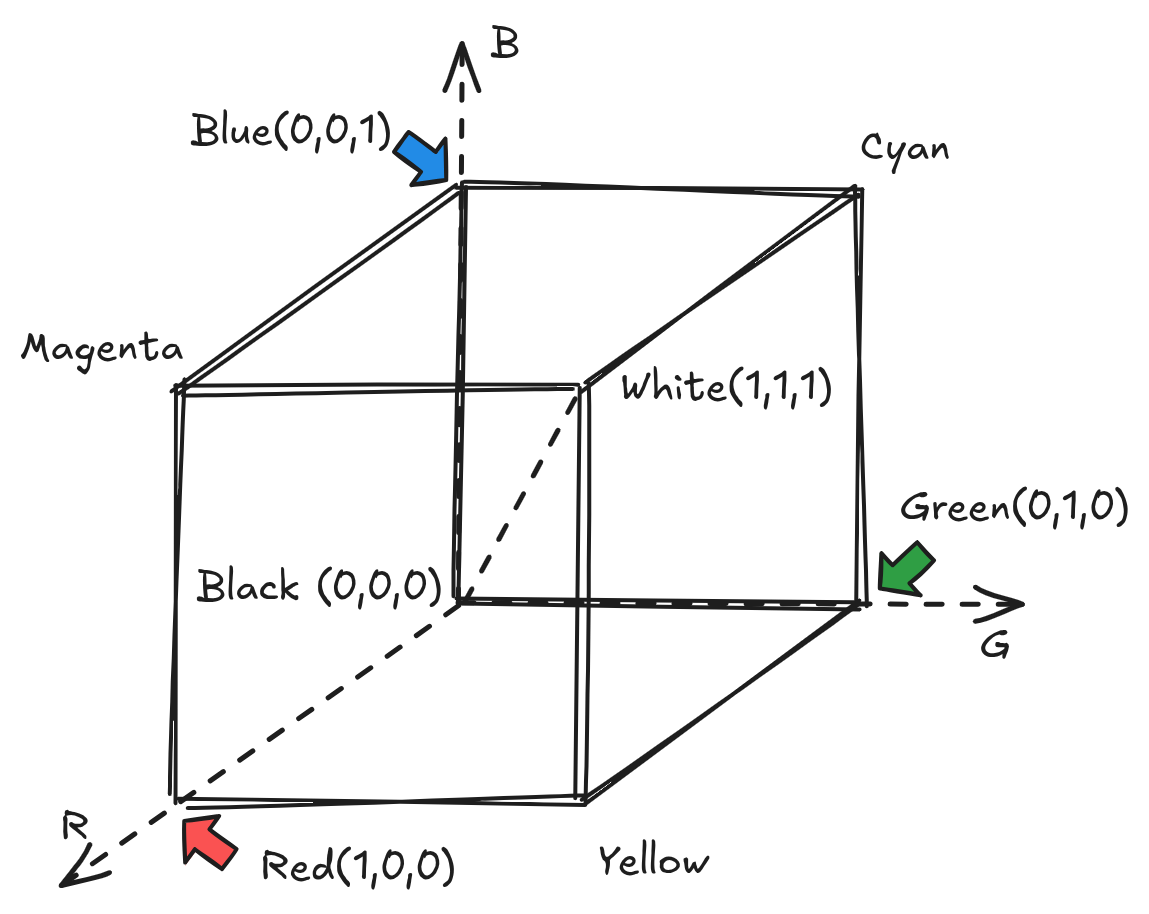
\includegraphics[width=12cm,angle=0]{rgb.png}};

\node at ($(current page.center)+(-12,8)$)
{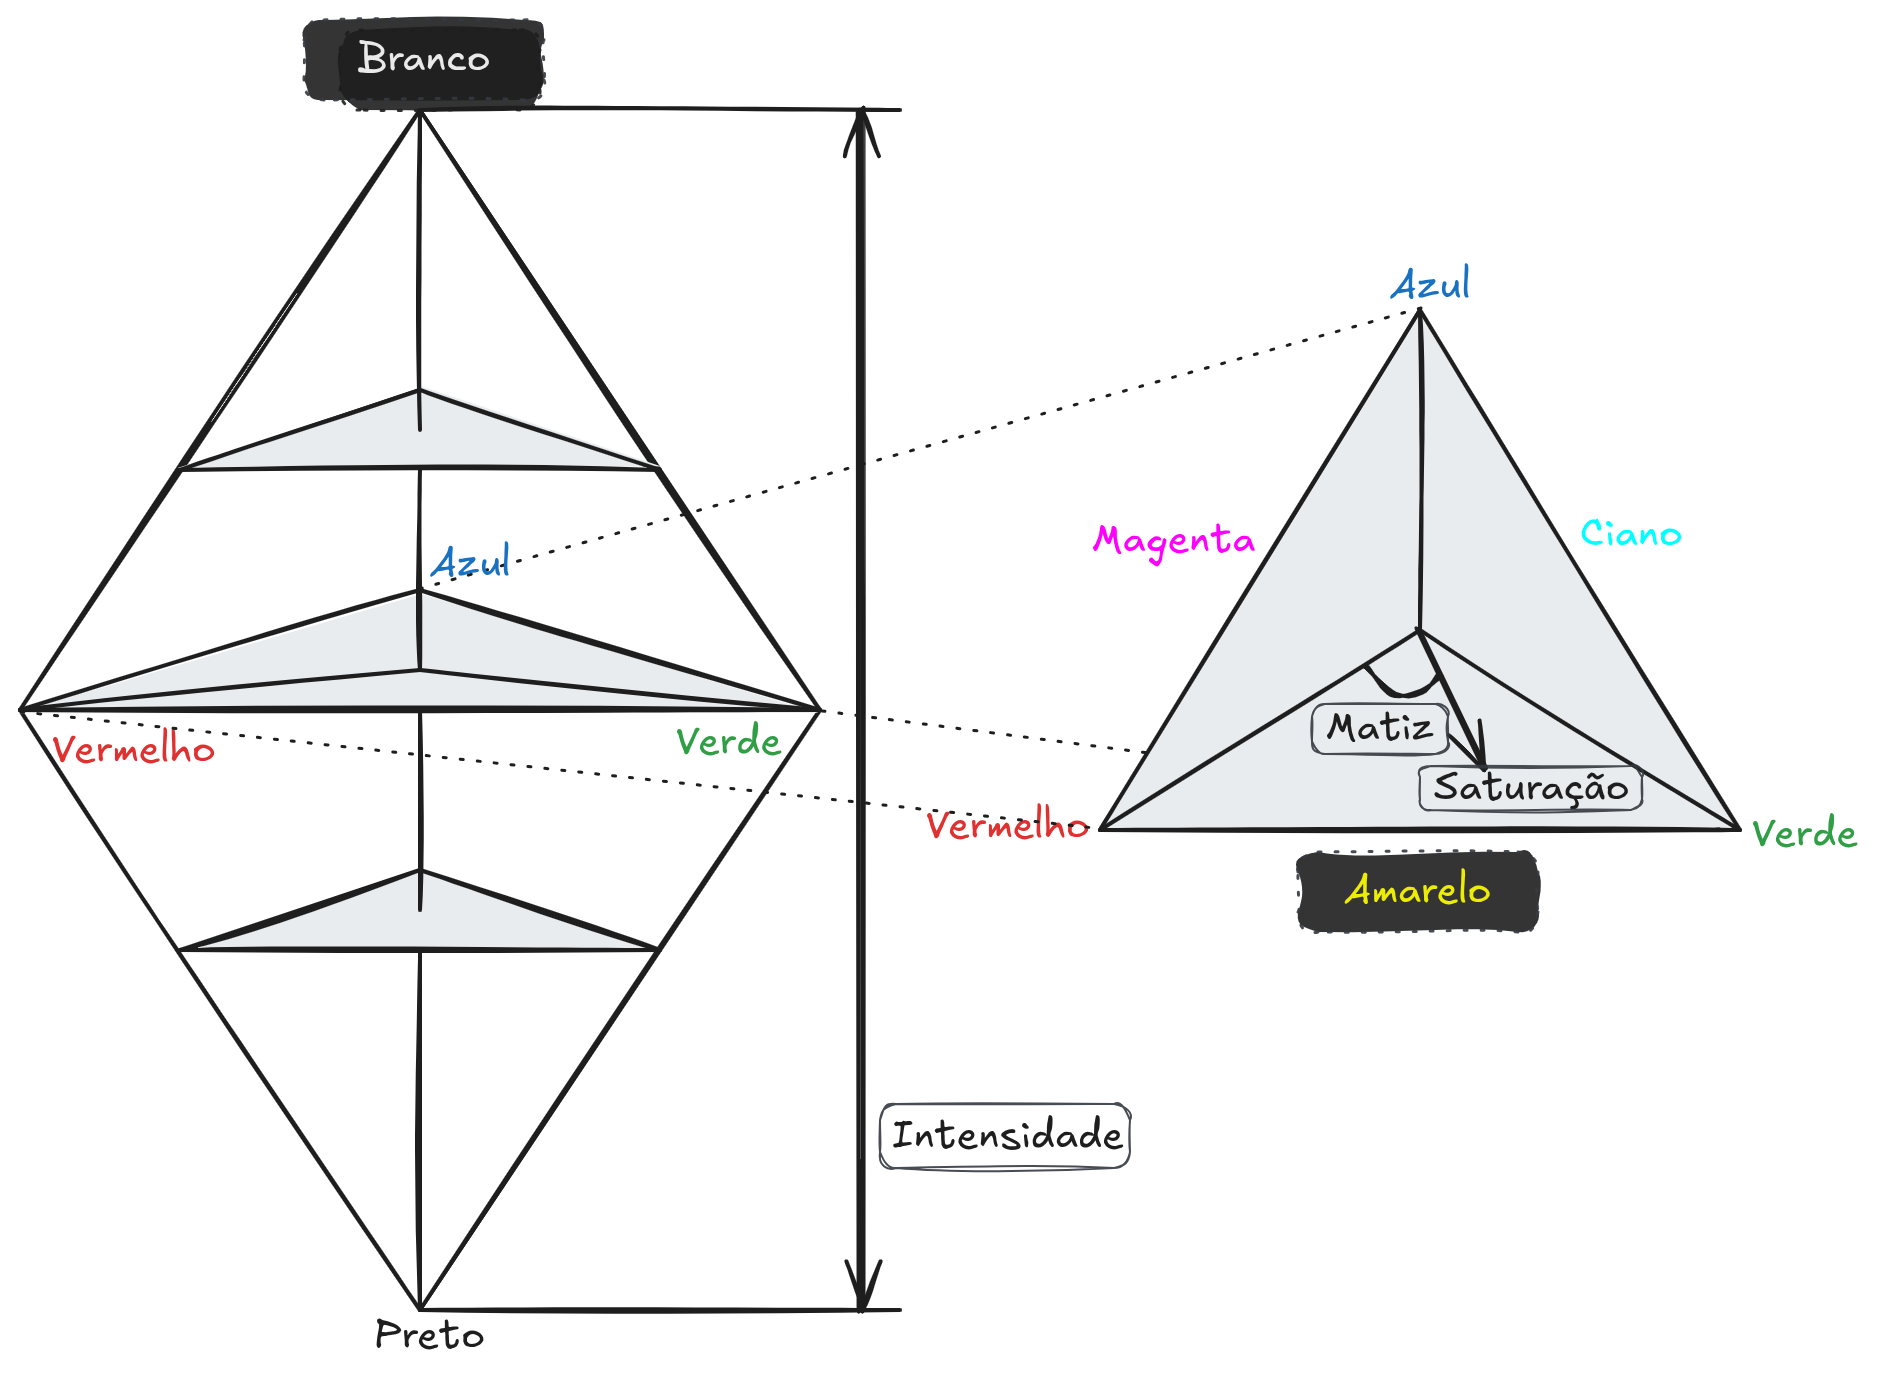
\includegraphics[width=12cm,angle=0]{hsi.png}};

\node at ($(current page.center)+(13,-9)$)
{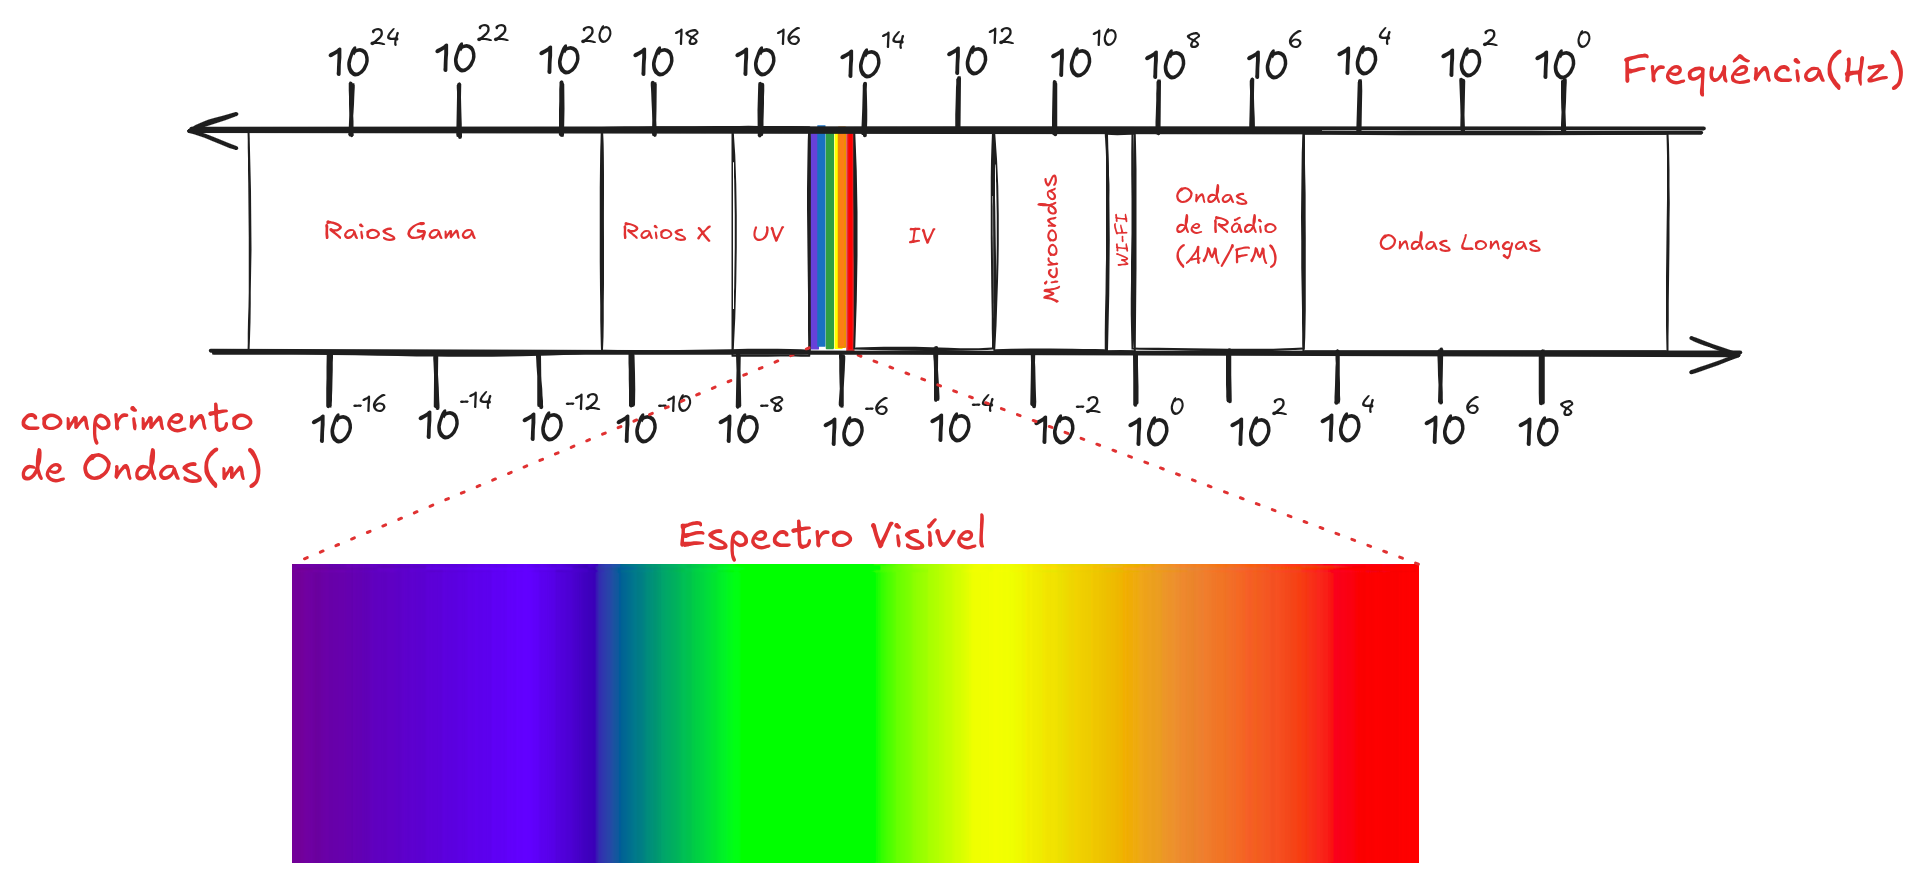
\includegraphics[width=16cm,angle=0]{espectro.png}};

\node at ($(current page.center)+(-12,-5)$)
{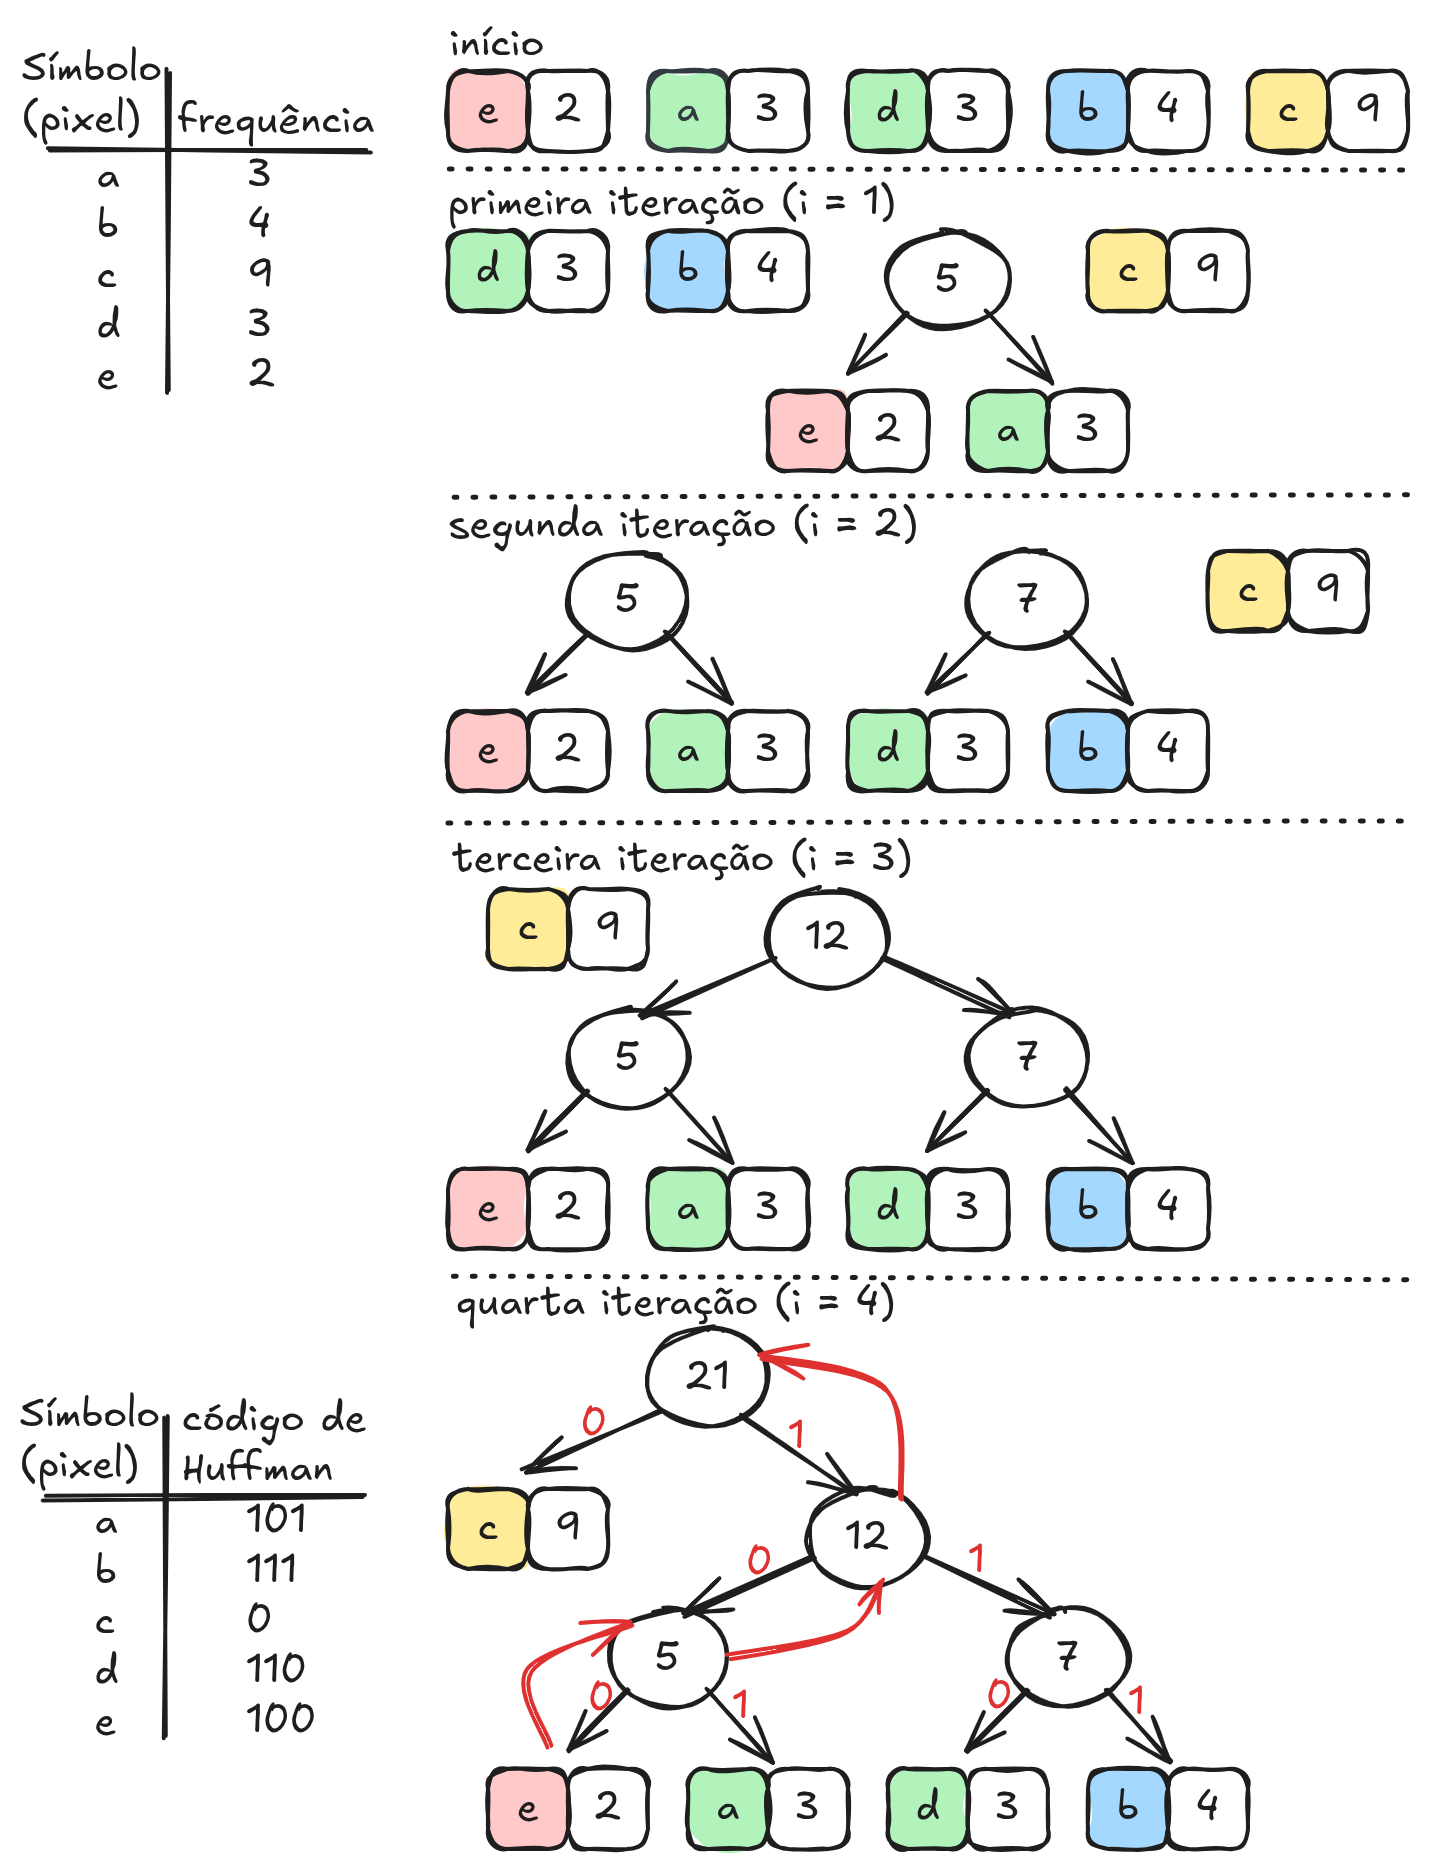
\includegraphics[width=12cm,angle=0]{huffman.png}};

% \node at ($(current page.center)+(0,7)$)
% {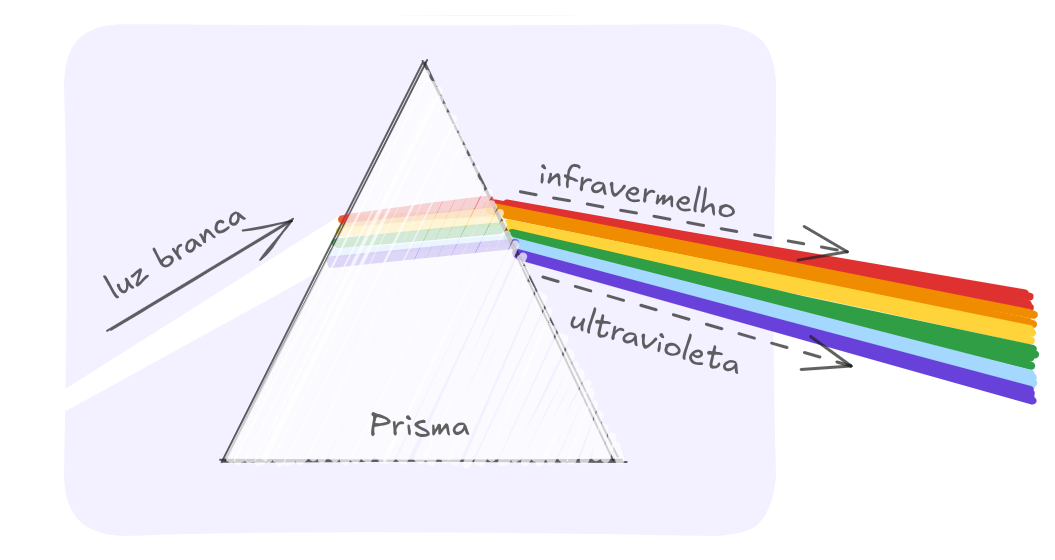
\includegraphics[width=14cm,angle=0]{prisma.png}};

\node at ($(current page.center)+(0,-7)$)
{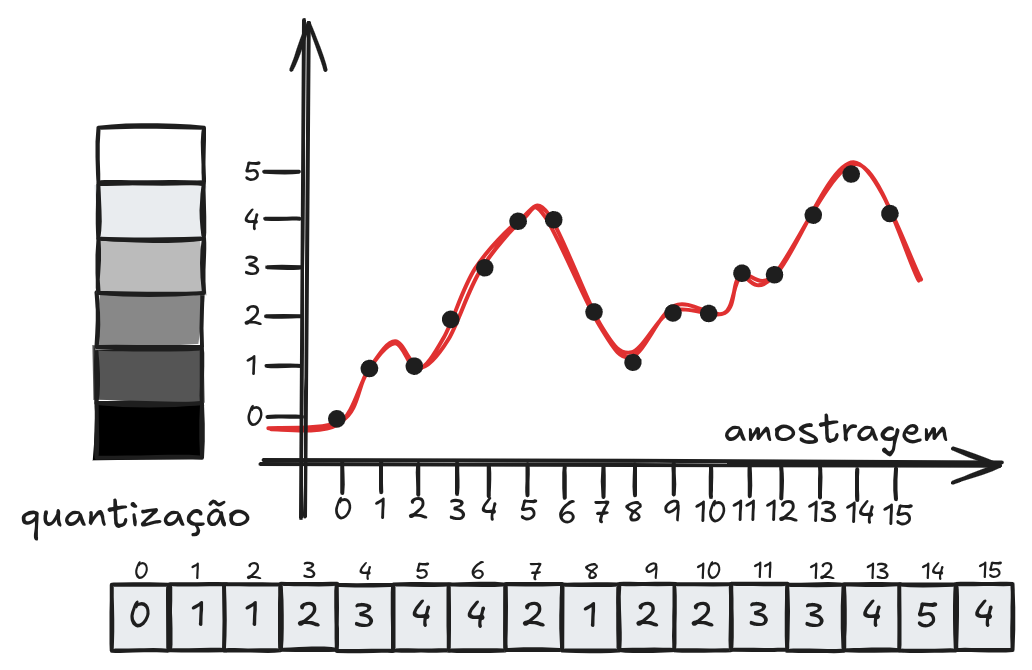
\includegraphics[width=9cm,angle=0]{amostragem.png}};

\node at ($(current page.center)+(13,0)$)
{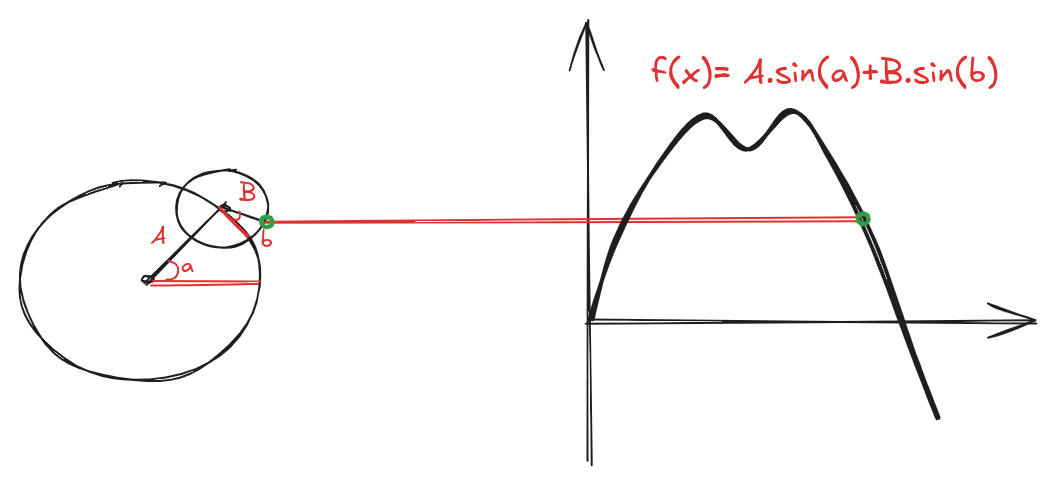
\includegraphics[width=14cm,angle=0]{epiciclo.png}};

\node at ($(current page.center)+(0,7)$)
{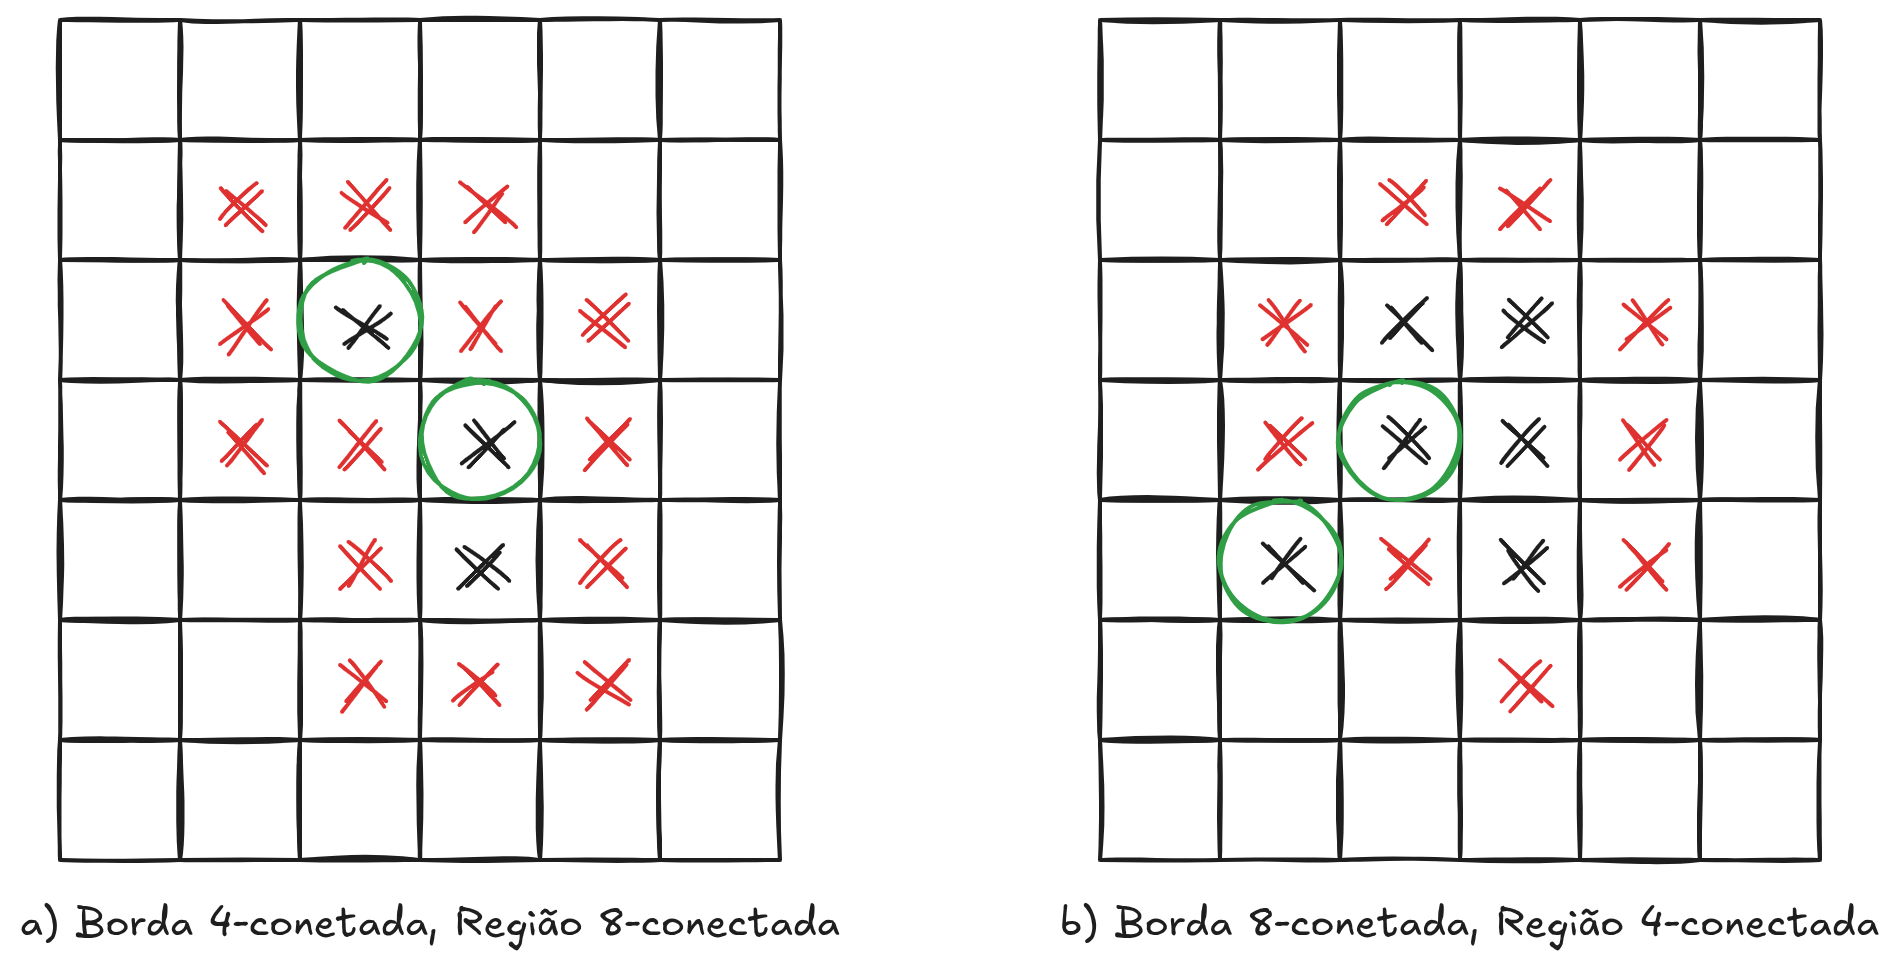
\includegraphics[width=10cm,angle=0]{paradoxo.png}};

\end{scope}

% =========================
% LOMBADA
% =========================
\node[rotate=90, text=black!80]
at (spine)
{\large Processamento Digital de Imagens};

% =========================
% CONTRACAPA
% =========================
\node[text=black!80, align=center]
at ($(back)+(0,0)$)
{
\small
Este livro apresenta conceitos fundamentais de\\
Processamento Digital de Imagens com abordagem\\
visual e interativa.\\[0.5cm]

Inclui exemplos práticos utilizando {\ttfamily p5.js}.
};

% ANO
\node[text=black!80]
at ($(back)+(0,-10)$)
{\small 2026};

\end{tikzpicture}

\end{document}